\chapter{ADQUISICIÓN DE LA INFORMACIÓN DE FASE}

Los sistemas ópticos tradicionales captan únicamente la información de la intensidad de la luz incidente sobre el sensor, perdiendo la información de fase, que resulta fundamental en aplicaciones, tales como, cristalografía de rayos-x \myfootcite{pinilla2018coded}, astronomía \myfootcite{fienup1987phase}, holografía \myfootcite{rivenson2018phase}, entre otras. Por lo tanto, la obtención de la información de fase  requiere la implementación  de sistemas ópticos que logren codificar la fase del campo óptico, preservándola implícita en las medidas de intensidad adquiridas. 
    
\section{SISTEMA ÓPTICO DE DIFRACCIÓN}
En múltiples áreas de la ciencia e ingeniería se presenta la adquisición de medidas de intensidad haciendo uso de sistemas ópticos de difracción \myfootcite{fienup1987phase,pinilla2018coded,rivenson2018phase}. La Figura \ref{fig:difraction_systems} muestra un esquema común de los sistemas ópticos de difracción, los cuales se componen por un objeto representado con el vector $\mathbf{z}$ iluminado por luz coherente, modulado en fase por una máscara de fase $\mathbf{D}$, produciendo las medidas cuadráticas codificadas. Dependiendo de la distancia del sensor $L$, la longitud de onda $\lambda$ y el radio de apertura $d$, los modelos de propagación se denominan campo cercano, medio y lejano.

\begin{figure}[h]
    \centering
    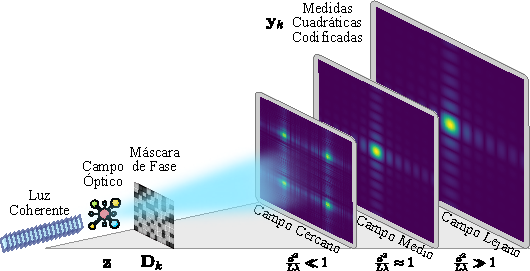
\includegraphics[width=\linewidth]{images/DiffractionSystem.pdf}
    \caption{\hspace{2mm}Sistema óptico codificado de difracción}
    \label{fig:difraction_systems}
\end{figure}

\section{PROBLEMA DE RECUPERACIÓN DE FASE}

Debido a que los sensores únicamente captan la información de la intensidad de la luz, el modelo de adquisición en los sistemas ópticos de difracción se describe como

\begin{equation}
    \mathbf{y}_{\ell, \psi} = \vert \mathbf{A}_{\ell, \psi}\mathbf{z} \vert^2, 
    \label{eq:phase_retrieval_problem}
\end{equation}

donde $\mathbf{z} \in {\mathbb{C}}^{n}$ es una vectorización del objeto de interés, $\mathbf{y}_{\ell, \psi} \in \mathbb{R}^{n}$ son las medidas adquiridas y $\mathbf{A}_{\ell, \psi}\in\mathbb{C}^{n\times n}$ son las matrices que describe la propagación en el campo $\psi$ del frente de onda de la luz hasta el sensor, con,  $\ell=1,\dots,L$, siendo $L$ el número total de proyecciones. De acuerdo con la teoría de difracción \myfootcite{poon2014introduction}, la propagación del frente de onda del objeto se modela entre los campos, cercano, medio y lejano dependiendo del número de Fresnel $F = \frac{d^2}{L\lambda}$, que determina el modelado matemático acorde a la zona de difracción en que se captan las medidas.

% \begin{align}
%     \mathbf{y}_k= 
%          \begin{cases}
%             \vert \mathbf{FTF}^{H}\mathbf{D}_k\mathbf{z} \vert^2, & \hfill (\text{Campo Cercano, }F \ll 1, \psi=1) \nonumber, \\ 
%             \vert \mathbf{F}^{H}\mathbf{Q}\mathbf{D}_k\mathbf{z} \vert^2,  & \hfill (\text{Campo Medio, }F \approx 1, \psi=2), \\
%             \vert \mathbf{F}\mathbf{D}_k\mathbf{z} \vert^2,  & \hfill (\text{Campo Lejano, } F \gg 1, \psi=3),   \nonumber
%          \end{cases}
%     \label{eq:modelado_zonas_difraccion}
% \end{align}

\begin{equation}
    \mathbf{y}_{\ell,\psi}= \left\{\begin{matrix}
\vert \mathbf{F}\mathbf{T}\mathbf{F}^\mathcal{H} \mathbf{D}_\ell \mathbf{z} \vert^2 & \text{si } \psi=1\rightarrow \text{Campo cercano}\\ 
\vert \mathbf{F}^\mathcal{H}\mathbf{Q}\mathbf{D}_\ell \mathbf{z} \vert^2&\text{si } \psi=2\rightarrow\text{ Campo medio} \\ 
\vert \mathbf{F}\mathbf{D}_\ell \mathbf{z} \vert^2 &\text{si } \psi=3\rightarrow\text{Campo lejano}
\end{matrix}\right., \label{eq:matrix_a}
\end{equation}

donde $\vert \cdot \vert$ representa el operador de magnitud, $\mathbf{F}$ corresponde a la transformada discreta de Fourier, la matriz diagonal $\mathbf{D}_\ell \in \mathbb{C}^{n \times n}$ representa las máscaras de fase, finalmente $\mathbf{T} \in \mathbb{C}^{n \times n}$ y $\mathbf{Q} \in \mathbb{C}^{n \times n}$ son matrices ortogonales que modelan la función de transferencia espacial del campo medio y cercano, respectivamente \myfootcite{poon2014introduction,goodman2005introduction}.

\begin{figure}[H]
    \centering
    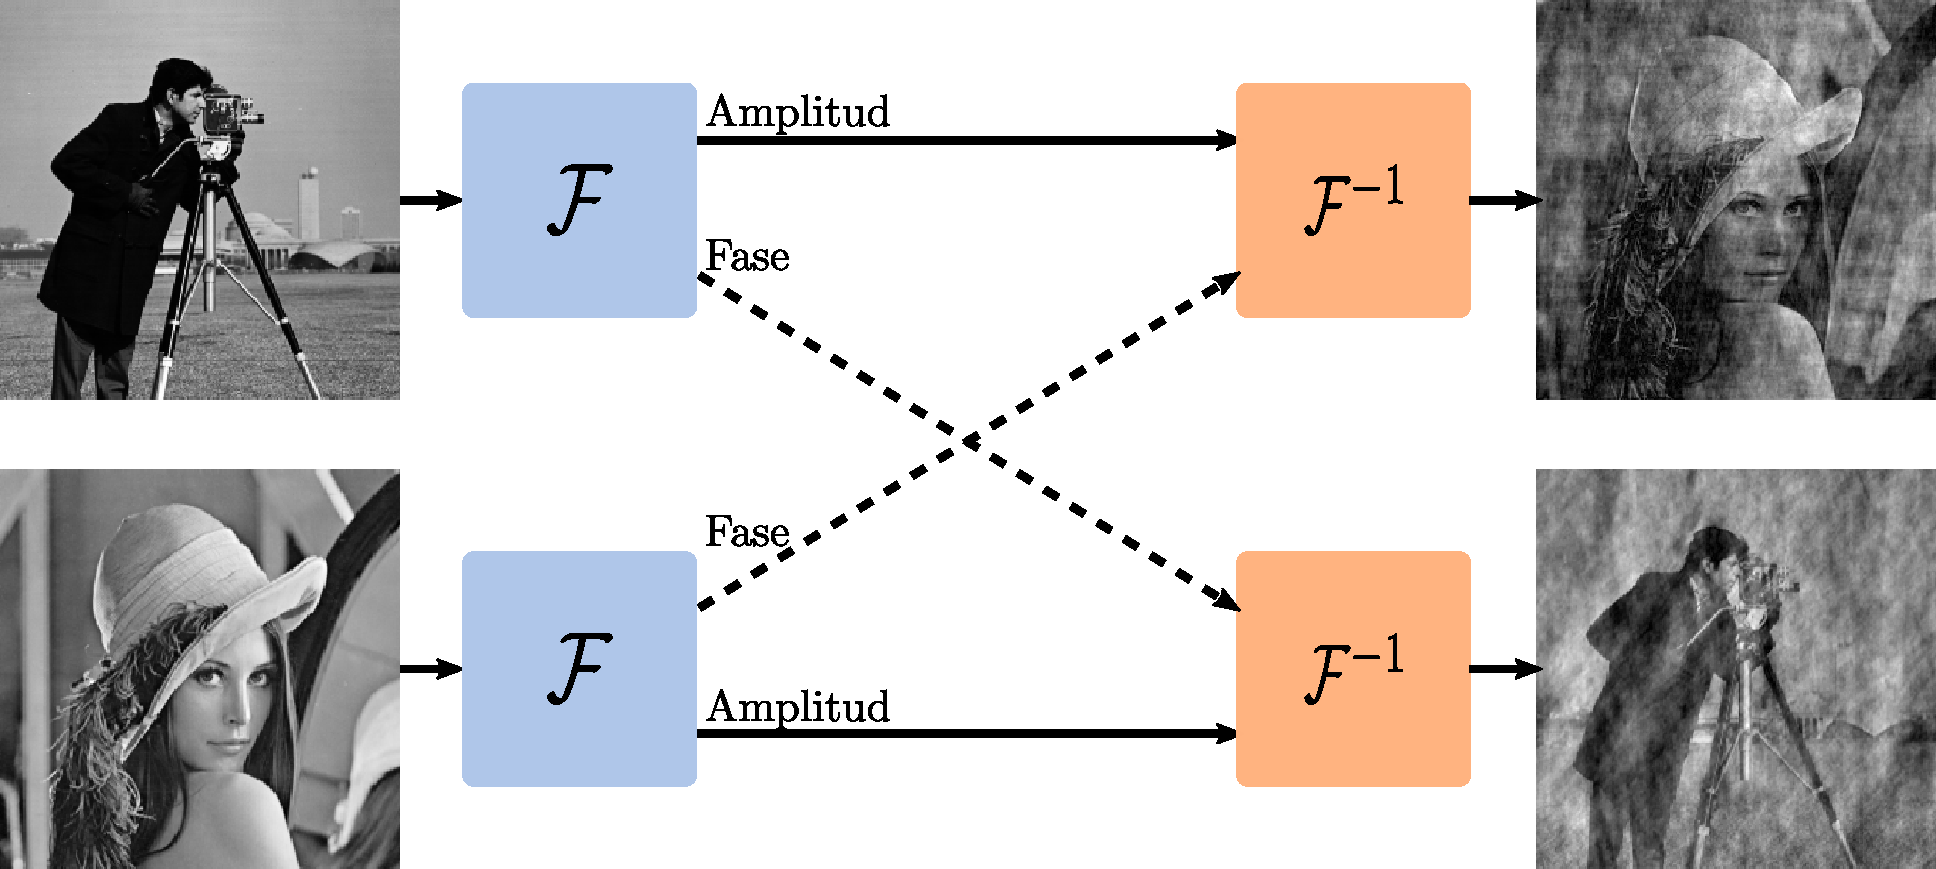
\includegraphics[width=0.8\linewidth]{images/mescla_abs_fase.pdf}
    \caption{\hspace{2mm}Experimento  intercambiando las fases de la transformada de Fourier de 2 imágenes .}
    \label{fig:mescla_fases}
\end{figure}

Cabe señalar la importancia de la información fase en Fourier a partir de la Figura \ref{fig:mescla_fases}. En esta Figura, se ilustra un experimento desarrollado en \myfootcite{shechtman2015phase} donde se intercambia la información de fase de la transformada de Fourier de dos imágenes, posteriormente, se aplica la transformada de Fourier inversa a este intercambio. En este ejemplo, se observa que en la imagen resultante predomina la información de las fases contrarias.

\section{MEDIDAS CUADRÁTICAS CODIFICADAS}
Dado la naturaleza cuadrática de la formulación en (\ref{eq:phase_retrieval_problem}), este problema se denomina como NP-difícil. Una forma de mitigar la complejidad de este problema, es incluyendo elementos de modulación de fase aleatorios en la formulación, puesto que, estas máscaras aleatorias permiten generar redundancia en las medidas, que conlleva a la obtención una solución exacta con alta probabilidad si se tienen las suficientes muestras \myfootcite{candes_CDP}.

Generalmente, las entradas aleatorias de la matriz  $\mathbf{D}_{\ell} = \mathrm{diag}(\mathbf{d})$ son $i.i.d$ copias de una variable aleatoria $d \in \mathbb{C}$ con $\mathbf{d} \in \{d\}^{n}$, donde $\mathrm{diag}(\cdot)$ devuelve una matriz diagonal cuadrada de un vector dado. Aquí, $d$ representa una modulación pasiva en la fase, se debe imponer que $d$ no aumenta la energía de la escena durante el proceso de modulación, por lo que se establece la Definición \ref{def:admissible}.

\begin{definition}{(Variable aleatorias admisible). \myfootcite{9062527}} 
    Una variable aleatoria que cumple con $|d|\leq 1$, se considera admisible como elemento de modulación en fase.\label{def:admissible}
\end{definition}


Algunos ejemplos de variables aleatorias que satisfacen la Definición \ref{def:admissible} se listan en la Tabla \ref{tab:admi_examples}. Estas variables aleatorias como elementos de codificación han sido usados en \myfootcite{9062527}.

\begin{table}[!h]
\centering
\begin{tabular}{|c|c|}
\hline
\textbf{Elemento de codificación} & \textbf{Probabilidad}                     \\ \hline
$d \in \{0, 1\}$         & $\{ \frac{1}{2},  \frac{1}{2}\}$ \\ \hline
$d \in \{-1, 1\}$        & $\{ \frac{1}{2},  \frac{1}{2}\}$ \\ \hline
$d \in \{-1, 1, -j,  j\}$ & $\{ \frac{1}{4},  \frac{1}{4}, \frac{1}{4},  \frac{1}{4}\}$ \\ \hline
\end{tabular}
\caption{Ejemplos de codificaciones aleatórias admisibles según la Definición \ref{def:admissible}.}
\label{tab:admi_examples}
\end{table}

% \begin{equation}
%     \vert d \vert \leq M, \quad \mathbb{E}[d] = 0, \quad  \mathbb{E}[d^2] = 0, \quad  \mathbb{E}[\vert d \vert^4] = 2\mathbb{E}[\vert d \vert^2]^2,    
%     \label{eq:restricciones_mascara}
% \end{equation}

% donde $\mathbb{E}[\cdot]$ corresponde al valor esperado. Aquí, se busca que $M=1$ para que la codificación no incremente la potencia de las medidas cuadráticas.

\chapter{ALGORITMOS DE RECUPERACIÓN DE FASE}
Para recuperar el campó óptico inicial a partir de medidas cuadráticas codificadas, la literatura ha planteado diferentes algoritmos basados en formulaciones convexas y no convexas.

\section{FORMULACIONES CONVEXAS}

Estos tipo de algoritmos relajan el problema recuperación de fase a un problema convexo equivalente.

\begin{itemize}
    \item \textbf{PhaseLift \myfootcite{candes2013phaselift}}:
    Este algoritmo plantea el problema de recuperación de la fase como una minimización de la traza de la siguiente forma
    \begin{equation}
        \begin{aligned}
            \minimize_{\mathbf{z} \in \mathbb{C}^{n}} \quad & \quad \mathrm{Traza}(\mathbf{z}\mathbf{z}^{\mathcal{H}}), \\
            \subjectto \quad & \quad \mathcal{A}(\mathbf{z}\mathbf{z}^{\mathcal{H}}) = \mathbf{b}, \\
             &\quad  \mathbf{z}\mathbf{z}^{\mathcal{H}} \succ 0,
        \end{aligned}
    \end{equation}
    
    donde $\mathcal{A}( \cdot ): \mathbb{R}^{n} \rightarrow \mathbb{R}^{m}$ es un operador lineal y $\mathrm{Traza}(\cdot)$ representa la traza de una matriz.
    
    \item \textbf{PhaseMax} \myfootcite{goldstein2018phasemax}:
    Sea $\mathbf{\hat{z}} \in \mathbb{C}^{n}$ un vector aproximación de la señal original $\mathbf{z}$, de modo que, la señal reconstruida se obtiene solucionando el siguiente problema convexo
        
    \begin{equation}
        \begin{aligned}
            \maximize_{\mathbf{z}\in \mathbb{C}^n} \quad & \langle \mathbf{z}, \mathbf{\hat{z}} \rangle_{\mathbb{R}}, \\
            \subjectto \quad & \vert \langle \mathbf{a}_i,\mathbf{z} \rangle \vert \leq (\boldsymbol{\phi})_i,
        \end{aligned}
    \end{equation}
    donde $\langle \cdot, \cdot \rangle_{\mathbb{R}}$ denota la parte real del producto interno y $(\boldsymbol{\phi})_i = \sqrt{(\mathbf{y})_i}$
    
\end{itemize}

\section{FORMULACIONES NO CONVEXAS}
Las formulaciones no convexas calculan el gradiente siguiendo la diferenciación de Wirtinger como los mostrados a continuación.
\begin{itemize}
    \item \textbf{TRUNCATED WIRTINGER FLOW (TWF):}
    El algoritmo TWF propuesto en \myfootcite{chen2017solving}, basa el modelo de muestreo según un variables aleatorias que siguen una distribución de Poisson de la forma:
    
    \begin{equation}
        (\mathbf{y})_i\sim \mathrm{Poisson}( \vert \langle \mathbf{a}_i,\mathbf{z}\rangle \vert^2 ), \quad i=1,\dots,m.
    \end{equation}
    
    TWF busca minimizar la máxima estimación de probabilidad 
    
    \begin{equation}
        \minimize_{z \in \mathbb{C}^{n}} - \sum_{i=1}^{m} \ell(\mathbf{z};\mathbf{y}_i),
    \end{equation}
    
    donde $\ell(\mathbf{z};\mathbf{y}_i) = { \mathbf{y}_i\log(|\mathbf{a}_i^H \mathbf{z}|^2) -|\mathbf{a}_i^H \mathbf{z}|^2 }$ con $(\cdot)^H$ el operador de conjugada transpuesta
    
    \item \textbf{TRUNCATED AMPLITUDE FLOW (TAF):}

    El algoritmo TAF \myfootcite{wang2017solving} adopta un criterio de mínimos cuadrados para recuperar $\mathbf{z}$ basado en las medidas sin fase $\mathbf{y}$ 
    
    \begin{equation}
        \minimize_{\mathbf{z} \in \mathbb{C}^{n}} \frac{1}{2m} \sum_{i=1}^{m} (\vert \langle \mathbf{a}_i,\mathbf{z}\rangle \vert - (\boldsymbol{\phi})_i)^2,
    \end{equation}
    
    Este algoritmo asume que las medidas $\mathbf{y}_i$ provienen de un sistema gaussiano de la forma $\mathbf{y}_i \sim \mathcal{N}(\vert \langle \mathbf{a}_i,\mathbf{z}\rangle \vert^2, 1)$
    
    \item \textbf{REWEIGHTED AMPLITUDE FLOW (RAF):}

    El algoritmo RAF formulado en \myfootcite{wang2018phase} sigue el criterio de maximizar la estimación de probabilidad de la forma
    
    \begin{equation}
        \minimize_{z \in \mathbb{C}^{n}} -\sum_{i=1}^{m} \ell(\mathbf{z};(\boldsymbol{\phi})_i/(\mathbf{y})_i),
    \end{equation}
    
    donde en el caso de un muestreo con ruido gaussiano basado en la amplitud $\ell(\mathbf{z};\mathbf{y}_i) = (\vert \langle \mathbf{a}_i,\mathbf{z}\rangle \vert - (\boldsymbol{\phi})_i)^2$ o basado en la intensidad  $\ell(\mathbf{z};(\mathbf{y})_i) = (\vert \langle \mathbf{a}_i,\mathbf{z}\rangle \vert^2 - (\mathbf{y})_i)^2$. Por otra parte, basado en un muestreo con distribución de Poisson, $\ell(\mathbf{z};(\mathbf{y})_i) = {(\mathbf{y})_i \log(|\mathbf{a}_i^H \mathbf{z}|^2) -|\mathbf{a}_i^H \mathbf{z}|^2 }$ 
\end{itemize}





\chapter{SISTEMAS DE CLASIFICACIÓN}

La clasificación ha sido una de las tareas computacionales más abordadas en el estado del arte. Específicamente, los algoritmos de clasificación se pueden separar en los más tradicionales como las SVM y KNN \myfootcite{kim12012comparing} y los algoritmos basados en redes neuronales que recientemente han dominado diferentes campos \myfootcite{li2019deep,li2018deep, wang2019development}
\section{MÁQUINAS DE SOPORTE VECTORIAL}
Las máquinas de soporte vectorial (SVM, por su sigla en inglés) \myfootcite{suthaharan2016support} son un método de clasificación binaria, donde cada punto $n$ dimensional $\mathbf{x}_i$ le corresponde una etiqueta de clase $c_i \in \{1,-1\}$.

Suponiendo que los datos de ambas clases son separables linealmente, este método propone separar los datos usando el hiper plano $\mathbf{w}\mathbf{x}_i + b = 0$. En la Figura \ref{fig:svm}, se muestra una representación de una SVM en $\mathbb{R}^2$

\begin{equation}
    \begin{split}
        \mathbf{w}\mathbf{x}_i + b &\geq 1 \quad si \quad c_i=1, \\
        \mathbf{w}\mathbf{x}_i + b &\leq 1 \quad si \quad c_i=-1.
    \end{split}
\end{equation}

Cabe resaltar que para todos los elementos del conjunto de datos se cumple que:

\begin{equation}
    c_i(\mathbf{w}\mathbf{x}_i + b) \geq 1, \quad i=1,\dots, m
\end{equation}

\begin{figure}[H]
    \centering
    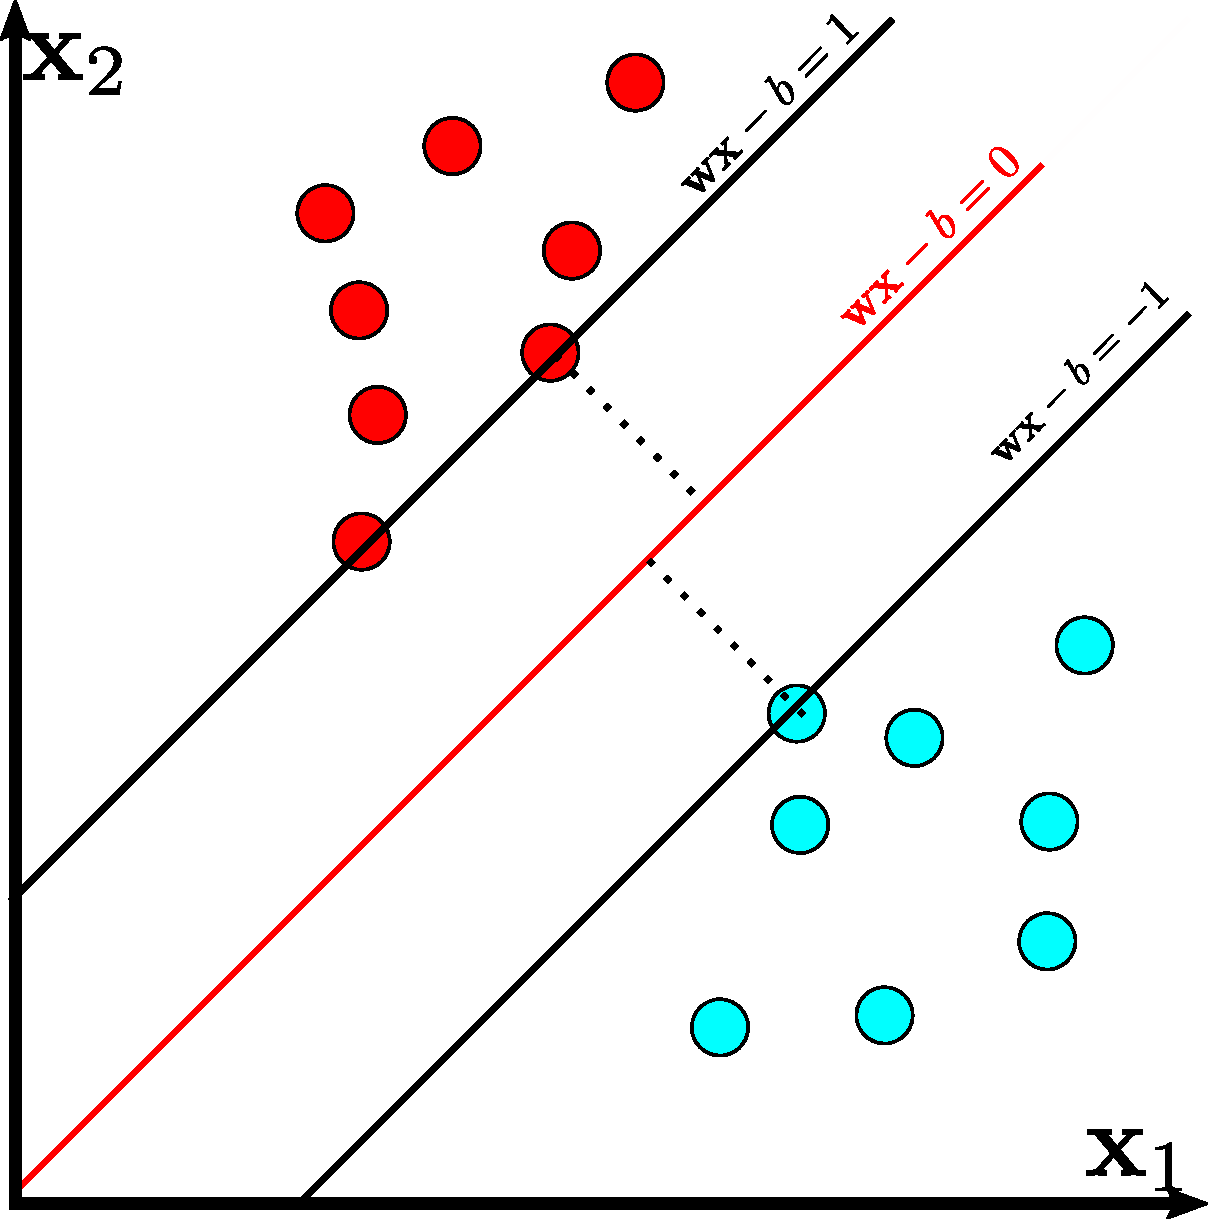
\includegraphics[width=0.4\linewidth]{images/svm.pdf}
    \caption{\hspace{2mm}Representación de una SVM en $\mathbb{R}^2$. La recta $\mathbf{wx} -b = 0$ en rojo representa el plano óptimo que soluciona el problema de optimización (\ref{eq:problema_optimización_svm}).}
    \label{fig:svm}
\end{figure}

El problema de optimización se plantea de la siguiente forma:

\begin{equation}
    \begin{aligned}
        \minimize_{\mathbf{w}} & \quad \Vert \mathbf{w} \Vert, \\
        \subjectto_{\quad i=1,\dots, m} & \quad c_i(\mathbf{w}\mathbf{x}_i + b) \geq 1.
    \end{aligned}
    \label{eq:problema_optimización_svm}
\end{equation}

Usualmente no es posible separar los datos linealmente, por esta razón, se puede incluir una función no lineal $ \phi$ que transforme los datos a un conjunto de características donde las clases sean separables linealmente. El problema de optimización para una SVM usando un kernel $\phi$ se formula como

\begin{equation}
    \begin{aligned}
        \minimize_{\mathbf{w}} & \quad \Vert \mathbf{w} \Vert, \\
        \subjectto_{\quad i=1,\dots, m} & \quad c_i(\mathbf{w}\phi(\mathbf{x}_i) + b) \geq 1.
    \end{aligned}
\end{equation}


\section{K VECINOS MÁS CERCANOS}

K vecinos más cercanos (KNN, por sus siglas en inglés) propone que un conjunto $D = \{(\mathbf{x}_i, c_i)\}_1^n$, siendo $\mathbf{x}_i$ el vector de características e $c_i$ la clase correspondiente. Para un nuevo vector a clasificar $\mathbf{\hat{x}}$, el algoritmo KNN encuentra los $K$ puntos más cercanos del dataset. La Figura \ref{fig:knn} muestra una representación de la clasificación de dos nuevas muestras en $\mathbb{R}^2$ con $K = 5$. Usualmente la función de distancia usada corresponde a la distancia euclidiana

\begin{equation}
    d(\mathbf{x}_p,\mathbf{x}_q) = \Vert \mathbf{x}_p-\mathbf{x}_q \Vert_2
    \label{eq:distancia_euclidiana}
\end{equation}

\begin{figure}[H]
    \centering
    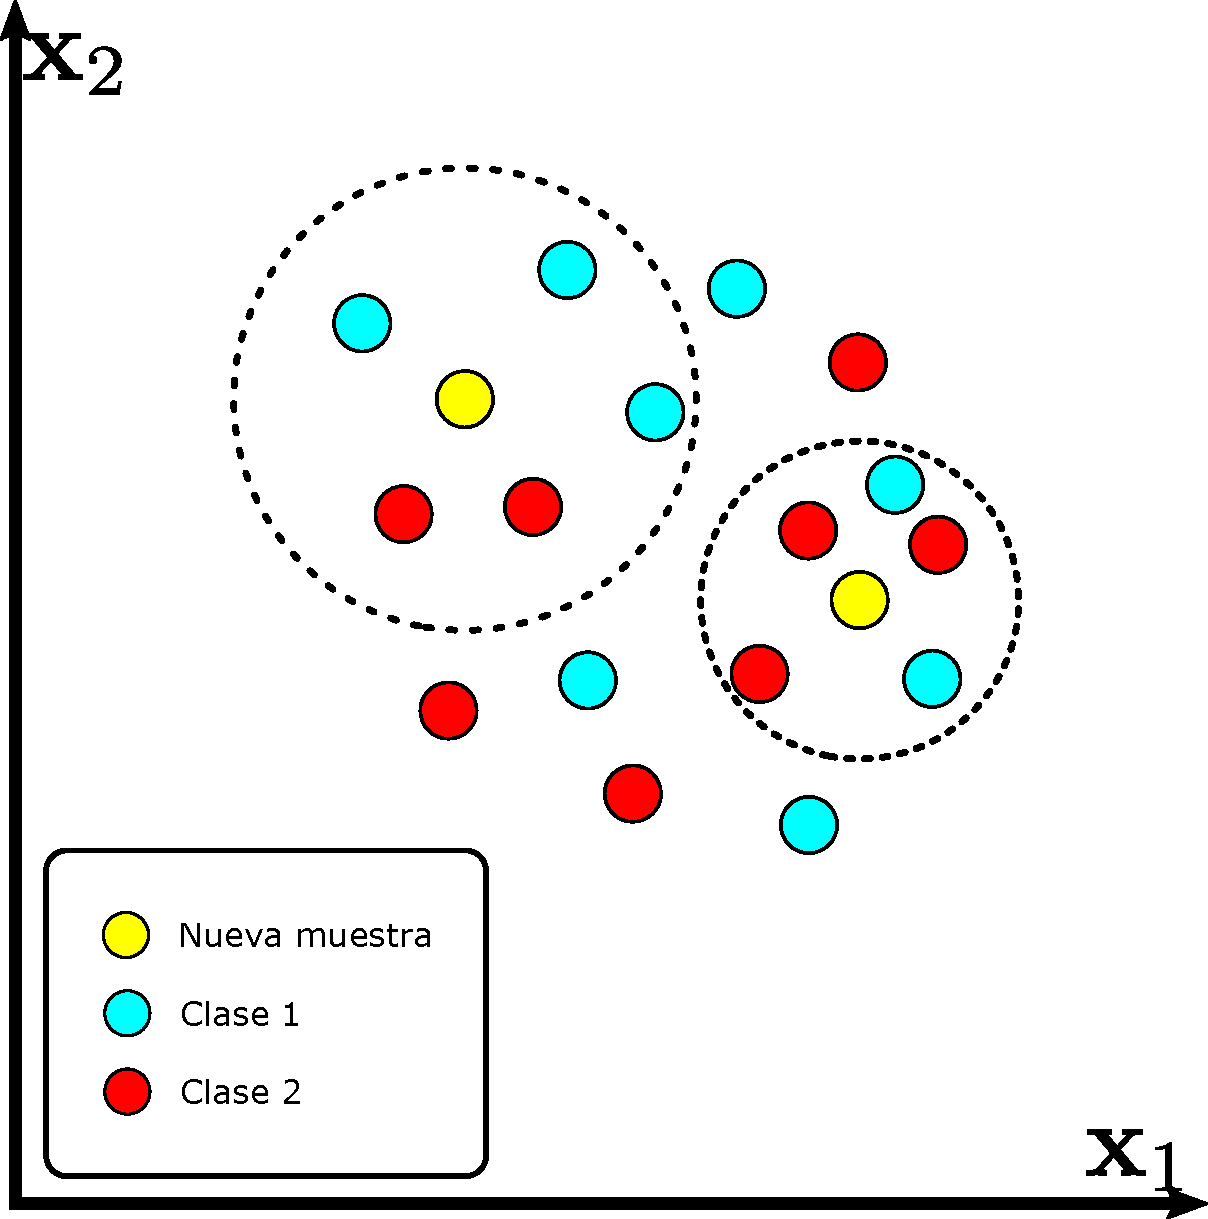
\includegraphics[width=0.4\linewidth]{images/knn.pdf}
    \caption{\hspace{2mm}Representación de KNN en $\mathbb{R}^2$ con $K = 5$.}
    \label{fig:knn}
\end{figure}

Posteriormente, haciendo uso de las clases de los $K$ puntos encontrados, de tal forma que $C \subset D$ y $\vert C \vert = K$, se cuantifica la cantidad de veces que aparece cada clase y se clasifica la nueva muestra $\mathbf{\hat{x}}$ con la clase que más veces aparezca de la forma

\begin{equation}
    \mathrm{clase}(\mathbf{\hat{x}}) =  \argmax_{\hat{c}} \bigg\{ \sum_{\hat{c} \in C} \delta(C,\hat{c})\bigg\},
\end{equation}

donde $\delta(\cdot,\cdot)$ corresponde a la función delta de Kronecker, dada por

\begin{equation}
    \delta(a,b) = \begin{cases}
        1, \quad a = b \\
        0, \quad a \neq b
    \end{cases}
\end{equation}
\section{REDES NEURONALES}

Los enfoques de aprendizaje profundo han generado un gran progreso en problemas muy complejos en los últimos años
\myfootcite{he2016deep,li2019deep,li2018deep, wang2019development,vaswani2017attention}. El aprendizaje profundo busca encontrar una función $f: \mathbb{R}^{d_1} \rightarrow \mathbb{R}^{d_2}$. La función $f$ se suele llamar arquitectura de red neuronal profunda, puesto que, consiste en la concatenación de múltiples capas compuestas de unidades mínimas llamadas neuronas. Cada neurona realiza una combinación lineal entre las entradas, para posteriormente usar una función no lineal en la salida. Las salidas de cada neurona en una capa funcionan como entrada de las neuronas ubicadas en la siguiente capa, creando así, una arquitectura de red neuronal profunda \myfootcite{fan2019selective}. En la Figura \ref{fig:nn}, se muestra una arquitectura de una arquitectura de red neuronal $f: \mathbb{R}^{d_1} \rightarrow \mathbb{R}^{d_2}$

\begin{figure}[H]
    \centering
    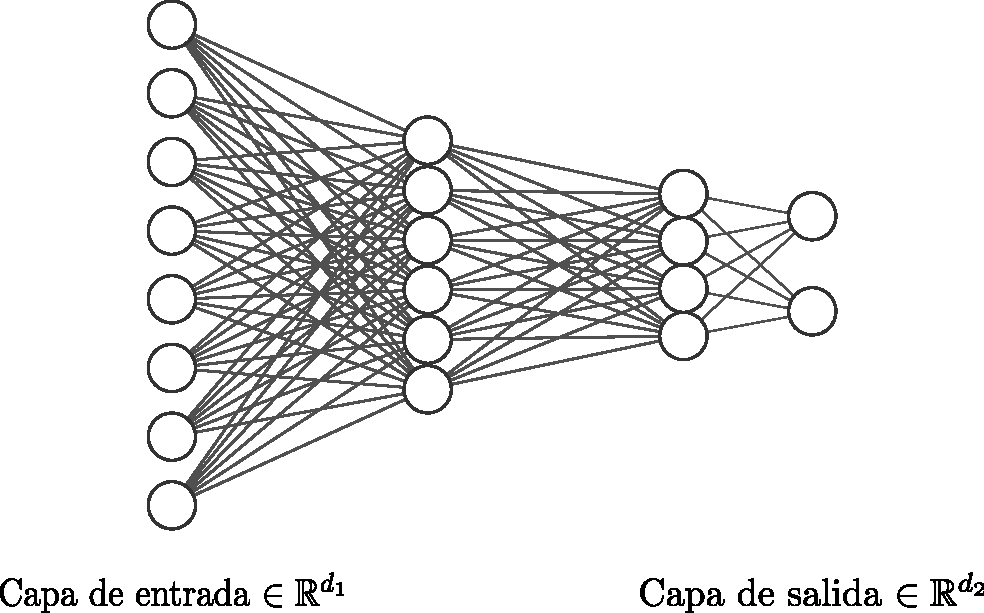
\includegraphics[width=0.6\linewidth]{images/nn.pdf}
    \caption{\hspace{2mm}Arquitectura de una arquitectura de red neuronal $f: \mathbb{R}^{d_1} \rightarrow \mathbb{R}^{d_2}$.}
    \label{fig:nn}
\end{figure}

En la ecuación. (\ref{eq:red_neuronal}), se muestra el modelado matemático de una red neuronal sencilla. 
\begin{equation}
    \footnotesize 
    \big\{f_\theta(\mathbf{x}) = \sigma_{L}(\mathbf{W}_{L}\sigma_{L-1}(\mathbf{W}_{L-1} (\dots \sigma_2(\mathbf{W}_2\sigma_1(\mathbf{W}_1\mathbf{x})))) \quad \vert \quad\theta = \{\mathbf{W}_{1} \dots \mathbf{W}_{L}\}  \big\},
    \label{eq:red_neuronal}
\end{equation}

donde para cada capa $1 \leq \ell \leq L$, $\sigma_\ell$ corresponde a una función no lineal en dicha capa y $\mathbf{W}_\ell$ La matriz de pesos. Para entrenar los pesos $\theta$ bajo un enfoque de aprendizaje supervisado, este método hace uso de un conjunto de entrenamiento $\{(\mathbf{x}_i, c_i) \}_{i=1}^{N}$ y una función de costo $\mathcal{L}( c_i,  f_\theta(\mathbf{x}_i))$ para plantear el problema de optimización 

\begin{equation}
    \minimize_\theta \frac{1}{N}\sum_{i=1}^{N} \mathcal{L}( c_i,  f_\theta(\mathbf{x}_i))
    \label{eq:optimización_nn}
\end{equation}

\section{CLASIFICACIÓN USANDO MEDIDAS CUADRÁTICAS}
En el campo de tomografía computarizada \myfootcite{douarre2020value} e imágenes de un solo píxel \myfootcite{bacca2020coupled}, se han propuesto sistemas de clasificación que usan únicamente medidas obtenidas a través del sistema lineal de adquisición, esto debido al enfoque basado en el aprendizaje profundo en el que la arquitectura incluye una capa con el sistema óptico de adquisición. Este enfoque ha sido estudiado igualmente en imágenes difractivas como en holografía \myfootcite{kim2018deep} y cristalografía de rayos-x \myfootcite{ziletti2018insightful}, donde las medidas obtenidas son difícilmente reconocidas por el ojo humano. 

Sin embargo, estos enfoques propuestos no han sido abordados en imágenes de medidas cuadráticas codificadas, de modo que, este trabajo propone el desarrollo de un algoritmo de clasificación usando medidas cuadráticas codificadas basado en aprendizaje profundo. 


\section{CLASIFICACIÓN DE IMÁGENES USANDO REDES NEURONALES ÓPTICAS}


Recientemente, se han publicado avances en el campo de redes neuronales implementadas físicamente haciendo uso de propiedades ópticas. Este tipo de redes resaltan debido al hecho que si se realiza la inferencia de manera óptica, la velocidad de cálculo está limitada por la velocidad de la luz en el medio y no requieren una fuente de energía activa para realizar los cálculos. Específicamente en \myfootcite{lin2018all} implementan las capas de una red neuronal haciendo uso de materiales difractados, realizando la modulación de la luz en la fase y aprovechando la propagación del campo óptico para realizar tareas de clasificación


\begin{figure}[!h]
    \centering
    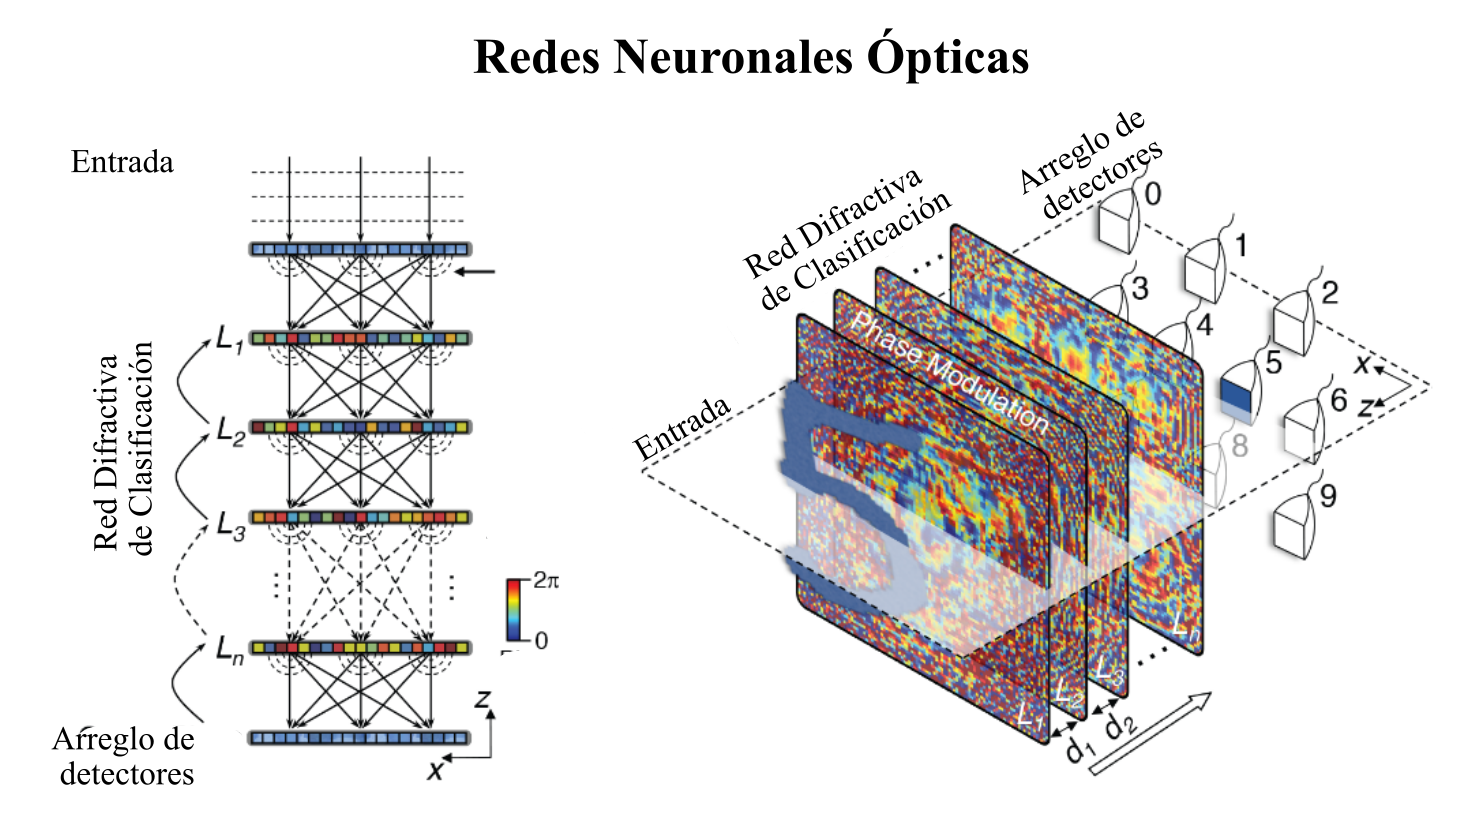
\includegraphics[width = 1\linewidth]{images/diffractive_networks.png}
    \caption{Implementación de redes neuronales ópticas implementadas ópticamente mediante elementos ópticos difractivos. Fuente: Modificado de \textit{All-optical machine learning using diffractive deep neural networks, 2018.}}
    \label{fig:optical_networks}
\end{figure}

